\section{Apparatus Required}
\markright{Apparatus Required}

\begin{table}[H]
    \centering
    \caption{Apparatus required for the experiment}
    \label{tab:lab2_apparatus}
    \renewcommand{\arraystretch}{1.45}
    \setlength{\tabcolsep}{10pt}
    \begin{tabular}{|c|p{0.34\textwidth}|p{0.38\textwidth}|}
        \hline
        \textbf{S. No.} & \textbf{Apparatus} & \textbf{Specification} \\
        \hline
        1 & P-n junction diode & 1N4007 silicon diode \\
        \hline
        2 & Regulated DC power supply & Variable DC output \\
        \hline
        3 & Resistor & $10\,\text{k}\Omega$ \\
        \hline
        4 & Ammeter & $0$--$20\,\text{mA}$ range \\
        \hline
        5 & Voltmeter & $0$--$20\,\text{V}$ range \\
        \hline
        6 & Breadboard & For temporary circuit construction \\
        \hline
        7 & Connecting wires & As required \\
        \hline
    \end{tabular}
\end{table}

\subsection*{Circuit Diagrams}

\begin{figure}[H]
    \centering
    \begin{subfigure}{0.48\textwidth}
        \centering
        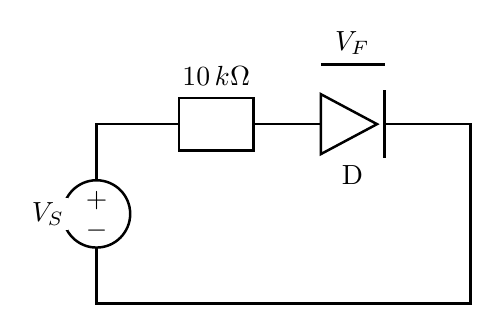
\begin{tikzpicture}[line width=0.9pt, scale=0.95, lablabel/.style={fill=white, inner sep=1.5pt}]
            \draw (0,0) circle (0.45);
            \node at (0,0.18) {$+$};
            \node at (0,-0.22) {$-$};
            \node[lablabel] at (-0.65,0) {$V_S$};
            \draw (0,0.45) -- (0,1.2) -- (1.1,1.2);
            \draw (1.1,0.85) rectangle (2.1,1.55);
            \node[lablabel] at (1.6,1.85) {$10\,\text{k}\Omega$};
            \draw (2.1,1.2) -- (3.0,1.2);
            \draw (3.0,0.8) -- (3.0,1.6) -- (3.75,1.2) -- cycle;
            \draw (3.85,0.75) -- (3.85,1.65);
            \node[lablabel] at (3.42,0.52) {D};
            \draw (3.85,1.2) -- (5.0,1.2) -- (5.0,-1.2) -- (0,-1.2) -- (0,-0.45);
            \draw (3.0,2.0) -- (3.85,2.0);
            \node[lablabel] at (3.42,2.28) {$V_F$};
        \end{tikzpicture}
        \caption{Forward bias}
        \label{fig:lab2_forward_circuit}
    \end{subfigure}
    \hfill
    \begin{subfigure}{0.48\textwidth}
        \centering
        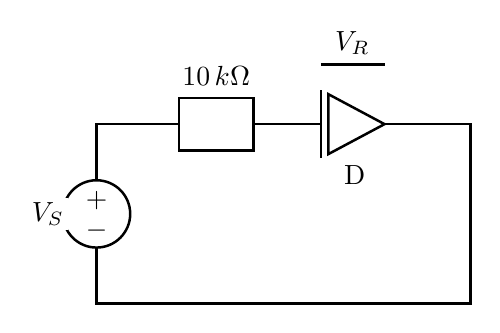
\begin{tikzpicture}[line width=0.9pt, scale=0.95, lablabel/.style={fill=white, inner sep=1.5pt}]
            \draw (0,0) circle (0.45);
            \node at (0,0.18) {$+$};
            \node at (0,-0.22) {$-$};
            \node[lablabel] at (-0.65,0) {$V_S$};
            \draw (0,0.45) -- (0,1.2) -- (1.1,1.2);
            \draw (1.1,0.85) rectangle (2.1,1.55);
            \node[lablabel] at (1.6,1.85) {$10\,\text{k}\Omega$};
            \draw (2.1,1.2) -- (3.0,1.2);
            \draw (3.0,0.75) -- (3.0,1.65);
            \draw (3.1,0.8) -- (3.1,1.6) -- (3.85,1.2) -- cycle;
            \node[lablabel] at (3.45,0.52) {D};
            \draw (3.85,1.2) -- (5.0,1.2) -- (5.0,-1.2) -- (0,-1.2) -- (0,-0.45);
            \draw (3.0,2.0) -- (3.85,2.0);
            \node[lablabel] at (3.42,2.28) {$V_R$};
        \end{tikzpicture}
        \caption{Reverse bias}
        \label{fig:lab2_reverse_circuit}
    \end{subfigure}
    \caption{Biasing circuits used to study the V--I characteristics of a p-n junction diode.}
    \label{fig:lab2_biasing_circuits}
\end{figure}
